\PassOptionsToPackage{unicode}{hyperref}
\PassOptionsToPackage{hyphens}{url}
\documentclass[
]{article}
\usepackage{lmodern}
\usepackage{amssymb,amsmath}
\usepackage{ifxetex,ifluatex}
\ifnum 0\ifxetex 1\fi\ifluatex 1\fi=0 % if pdftex
  \usepackage[T1]{fontenc}
  \usepackage[utf8]{inputenc}
  \usepackage{textcomp} % provide euro and other symbols
\else % if luatex or xetex
  \usepackage{unicode-math}
  \usepackage{hyperref}
  \usepackage{verbatim}
  \defaultfontfeatures{Scale=MatchLowercase}
  \defaultfontfeatures[\rmfamily]{Ligatures=TeX,Scale=1}
\fi
% Use upquote if available, for straight quotes in verbatim environments
\IfFileExists{upquote.sty}{\usepackage{upquote}}{}
\IfFileExists{microtype.sty}{% use microtype if available
  \usepackage[]{microtype}
  \UseMicrotypeSet[protrusion]{basicmath} % disable protrusion for tt fonts
}{}
\makeatletter
\@ifundefined{KOMAClassName}{% if non-KOMA class
  \IfFileExists{parskip.sty}{%
    \usepackage{parskip}
  }{% else
    \setlength{\parindent}{0pt}
    \setlength{\parskip}{6pt plus 2pt minus 1pt}}
}{% if KOMA class
  \KOMAoptions{parskip=half}}
\makeatother
\usepackage{xcolor}
\IfFileExists{xurl.sty}{\usepackage{xurl}}{} % add URL line breaks if available
\IfFileExists{bookmark.sty}{\usepackage{bookmark}}{\usepackage{hyperref}}
\hypersetup{
  hidelinks,
  pdfcreator={LaTeX via pandoc}}
\urlstyle{same} % disable monospaced font for URLs
\usepackage{graphicx}
\makeatletter
\def\maxwidth{\ifdim\Gin@nat@width>\linewidth\linewidth\else\Gin@nat@width\fi}
\def\maxheight{\ifdim\Gin@nat@height>\textheight\textheight\else\Gin@nat@height\fi}
\makeatother
% Scale images if necessary, so that they will not overflow the page
% margins by default, and it is still possible to overwrite the defaults
% using explicit options in \includegraphics[width, height, ...]{}
\setkeys{Gin}{width=\maxwidth,height=\maxheight,keepaspectratio}
% Set default figure placement to htbp
\makeatletter
\def\fps@figure{htbp}
\makeatother
\setlength{\emergencystretch}{3em} % prevent overfull lines
\providecommand{\tightlist}{%
  \setlength{\itemsep}{0pt}\setlength{\parskip}{0pt}}
\setcounter{secnumdepth}{-\maxdimen} % remove section numbering

\author{Duong Tung}
\date{\today}

\begin{document}
\begin{center}
    \textbf{Group:} 16\\
    \textbf{Students: } Duong Doan Tung, Pham Van Cong, Le Hoang Nam\\
    
    \textbf{Course:} Applied Mathematics for Artificial Intelligence\\

\end{center}
\textbf{Assignment 4}\\
This latex only cover part 3 of Assignment, for other parts please refer to Assignment4.ipynb file on google colab.\\
\textbf{Hyper link to google colab notebook: }\href{https://colab.research.google.com/github/dtungpka/Applied-Mathematics-for-Artificial-Intelligence/blob/dev/Assignment_4/Assignment%204.ipynb}{Assignment 4.ipynb}\\
\textbf{Hyper link to github repository: }\href{https://github.com/dtungpka/Applied-Mathematics-for-Artificial-Intelligence/tree/dev/Assignment_4}{Assignment 4}\\
\section{Part 3}
\subsection{Problem 1}


We define that:\\
\begin{enumerate}
A is "Test positive"\\
B is "Has Ebola"\\\\
\end{enumerate}
According to the problem, we have:\\
P(A|B) = $84\%$\\
P($A|\overline{B}$) = 11\%\\
P(B) = 0.9\%\\ \\
If a random person is tested positive, the probability that he/she actually has Ebola is:\\
\begin{array}{rcl}
    P(B|A) & = & \frac{P(A|B)\cdot P(B) }{P(A)} \\
     & = & \frac{P(A|B)\cdot P(B)}{P(A|B)\cdot P(B)+P(A|\overline{B})\cdot P(\overline{B})} \\
     & = &\frac{P(A|B)\cdot P(B)}{P(A|B)\cdot P(B)+P(A|\overline{B})\cdot (1- P(B))} \\
    & = &\frac{84\%\cdot 0,4\%}{84\%\cdot 0,4\%+11\%\cdot (1- 0,4\%)}\\
    & = & 2,98\%
    \end{array}



\subsection{Problem 2}

We define that:\\
\begin{enumerate}
A is "players type 1"\\
B is "players type 2"\\
C is "players type 3"\\
W is "winning a game"\\\\
\end{enumerate}
According to the problem, we have:\\
P(A) = $0,5$\\
P(B) = 0,25\\
P(B) = 0,25\\\\
P(W|A) =  0,3\\
P(W|B) =  0,4\\
P(W|C) =  0,5\\\\

(A)
The probability of winning against a random player is:\\
\begin{array}{rcl}
    P(W)& = &P(W|A)\cdot P(A) + P(W|B)\cdot P(B) + P(W|C)\cdot P(C)\\
& = & 0,3\cdot 0,5 + 0,4\cdot 0,25 + 0,5\cdot 0,25\\
& = & 0,375

\end{array}\\
(B)The probability of winning against a player of type 1 is:\\
\begin{array}{rcl}
    P(W|A)& = &\frac{P(W|A)\cdot P(A)}{P(W)}\\
& = & \frac{0,3\cdot 0,5}{0,375}\\
& = & 0,4

\end{array}\\


\subsection{Problem 3}
Sample space: \\
$ \Omega = {red, green, blue,orange, yellow}$\\
(A) The smallest possible vaild event space \mathcal{A}  is:\\
\begin{array}{rcl}
    \mathcal{A} & = & \{ \emptyset,\{red, green, blue, orange, yellow\} \} \\
\end{array}\\\\
(B) Smallest possible event space that contains the event set \{blue\} is:\\
\begin{array}{rcl}
    \mathcal{B} & = & \{ \emptyset,\{blue\},\{red, green, blue, orange, yellow\} \} \\
\end{array}\\\\
(C) Smallest possible event space that contains both the event set \{blue\} and \{red, green\} is:\\

   $ \mathcal{C}  =  \{ \emptyset,\{blue\},\{red, green\},\{orange,yellow\},\{blue,orange,yellow\},\{red,green,blue\},\\\{red,green,orange,yellow\},\{red, green, blue, orange, yellow\} \} \\$
\newpage
\subsection{Problem 4}
%include img i1.png
\begin{figure}[htbp]
\centering
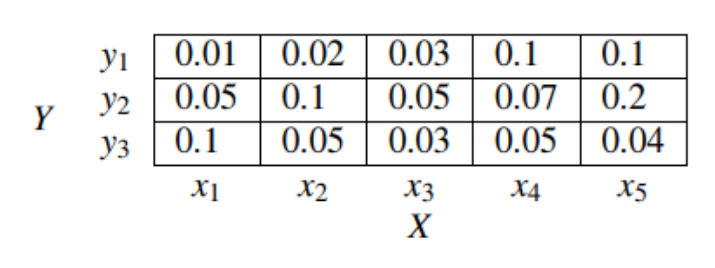
\includegraphics[width=0.5\textwidth]{i1.png}
\caption{Problem 4}
\end{figure}
(A) Marginal distribution of X is:\\
\begin{tabular}{|c|c|c|c|c|c|}
\hline
X & 1 & 2 & 3 & 4 & 5\\
\hline
P(X) & 0.16 & 0.17 & 0.11 & 0.22 & 0.34\\
\hline
\end{tabular}\\\\
(B) Marginal distribution of Y is:\\
\begin{tabular}{|c|c|c|c|}
\hline
Y & 1 & 2 & 3\\
\hline
P(Y) & 0.26 & 0.47 & 0.27\\
\hline
\end{tabular}\\

(C) Conditional distribution of X given Y $= y_1$ is:\\
$P(X|Y=1) = \frac{P(X,y_1)}{P(y_1)}, $\\
\begin{tabular}{|c|c|c|c|c|c|}
\hline
X & 1 & 2 & 3 & 4 & 5\\
\hline
P(X|Y=1) & $\frac{1}{26}$  & $\frac{1}{13}$ & $\frac{3}{26}$ & $\frac{5}{13}$ & $\frac{5}{13}$\\
\hline
\end{tabular}\\\\
(D) Conditional distribution of Y given X $= x_3$ is:\\
$P(Y|x_3) = \frac{P(x_3,Y)}{P(x_3)}, $\\
\begin{tabular}{|c|c|c|c|}
\hline
Y & 1 & 2 & 3\\
\hline
P(Y|x_3) & $\frac{3}{11}$  & $\frac{5}{11}$ & $\frac{3}{11}$\\
\hline
\end{tabular}\\

(E) Conditional distribution of X given Y $\neq y_1$ is:\\
$P(X|Y\neq y_1) = \frac{P(X,Y=y_{23})}{P(Y=y_{23})}, $\\
\begin{tabular}{|c|c|c|c|c|c|}
\hline
X & 1 & 2 & 3 & 4 & 5\\
\hline
P(X|Y\neq y_1) & $\frac{15}{74}$  & $\frac{15}{74}$ & $\frac{4}{37}$ & $\frac{6}{37}$ & $\frac{12}{37}$\\
\hline
\end{tabular}\\

\subsection{Problem 5}
The solution for this problem is in the attached ipynb file.
\end{document}
